\chapter{Introduction}
\label{chap:intro}
\minitoc

% This work aims to use a Hyperspectral Imaging (HSI) camera to extract semantic and physiologically relevant data in real-time during neuro-oncological surgery. These data are expected to aid decision-making, thereby reducing cognitive workload for the surgeons without compromising patient outcomes. The following introduction summarises the fundamentals of brain tumours and current operating practice.  This is followed by a summary of Hyperspectral Imaging, key data post-processing steps, and an outline of the thesis.

\section{Hyperspectral imaging}
Hyperspectral imaging (HSI) measures diffuse reflectance spectra using multiple channels, which are narrow spectral measurements centred around a given wavelength. In comparison, traditional imaging only collects three broad channels to create a conventional RGB (red, green, blue) image. This provides higher spectral resolution than traditional imaging whilst maintaining a wide field of view. This technique can also
be referred to as multispectral imaging when there is a low number of bands, however for simplicity we will refer to this as HSI in all cases~\cite{Clancy2020}.

There are three major categories of HSI cameras: spatial scanning, spectral scanning, and snapshot acquisition. Spatial scanning collects data for all wavelengths simultaneously and scans through pixels sequentially, these can be sub-categorised by the scanning order such as linescan or pointscan. Spectral scanning, however, acquires data for all pixels simultaneously and scans through wavelengths sequentially. These methods both capture data consisting of two spatial and one spectral axes directly, forming a full hypercube. In contrast, snapshot aquisition instead acquires one channel per pixel in a single shot~\cite{Geelen2014} with the remaining data inferred by classical or learning-based~\cite{Li2021} interpolation (demosaicing) to construct a full hypercube. Following this demosaicing step, a spectral cross-talk correction must be performed as these systems suffer from parasitic neighbouring channel effects~\cite{Pichette2017}. These acquisition types are represented in Figure \ref{fig:scanning}. 
\begin{figure}[h]
    \centering
    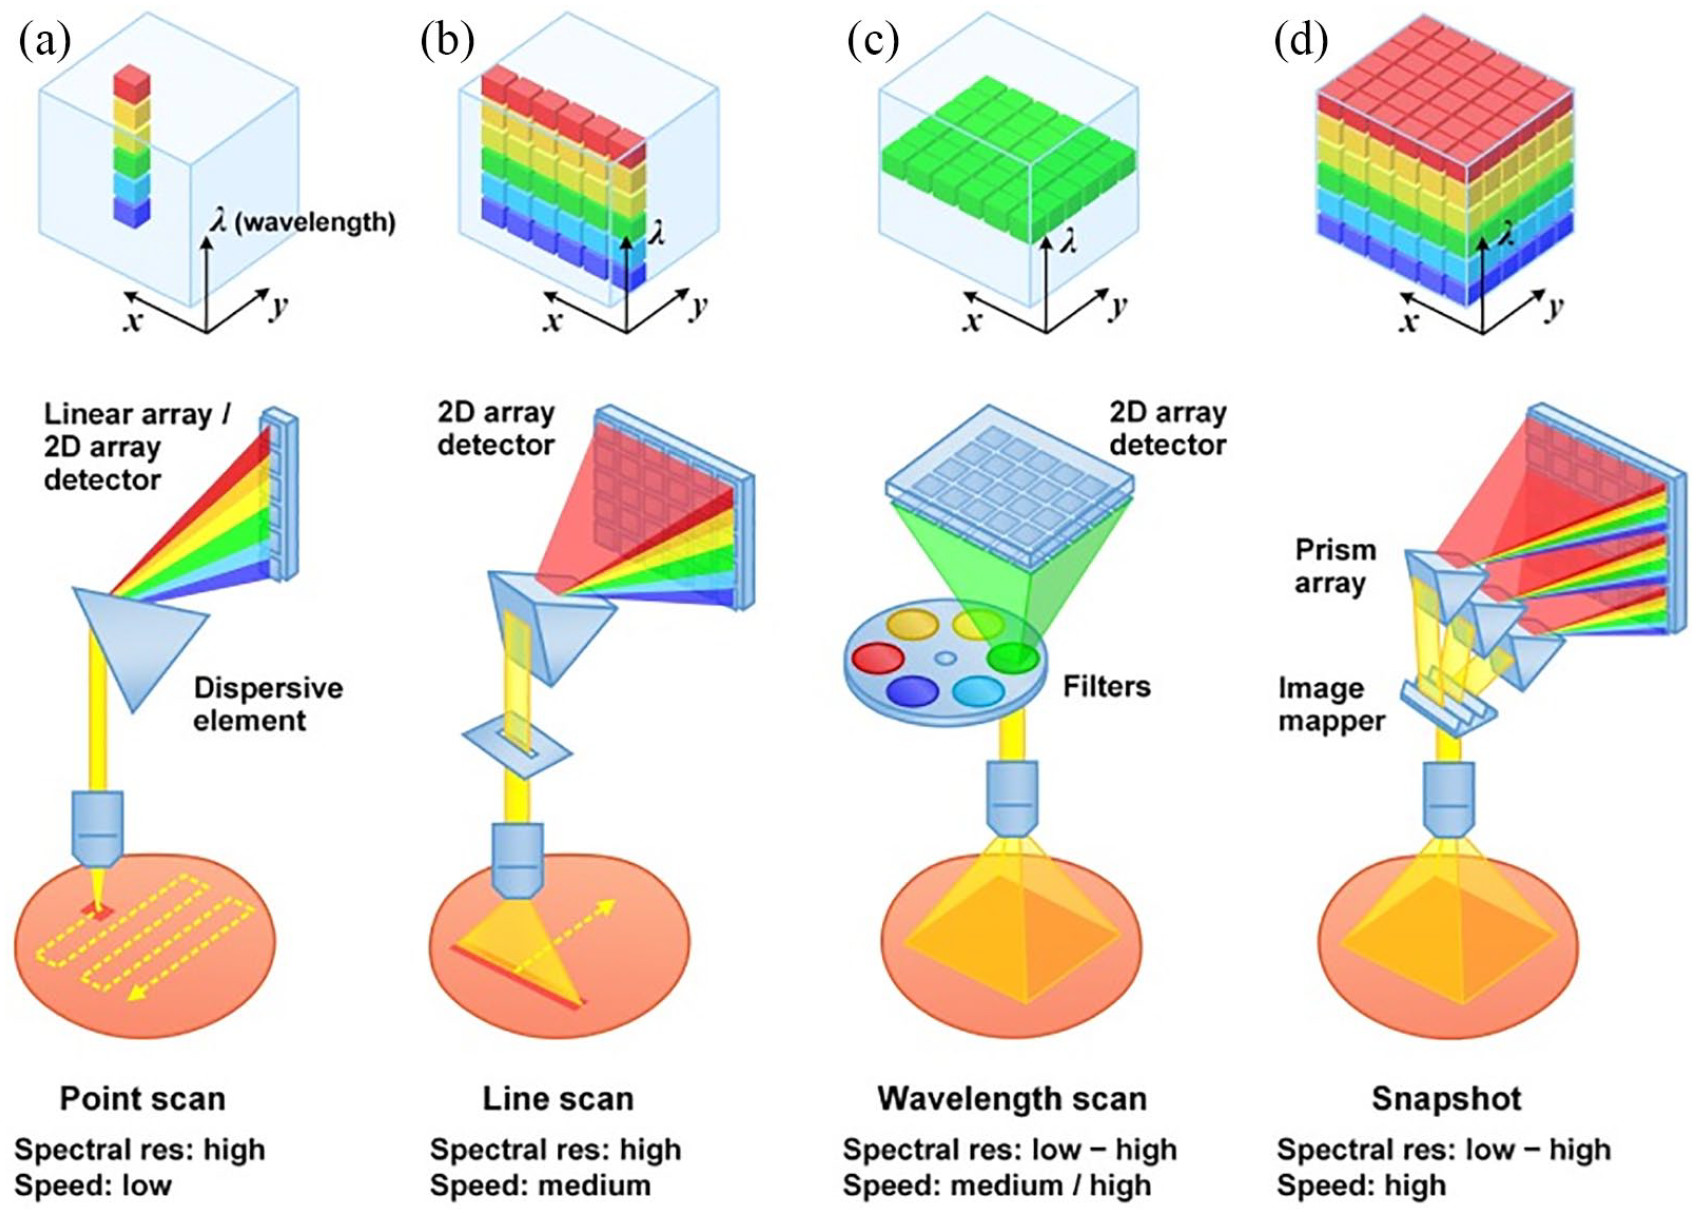
\includegraphics[width=0.7\textwidth]{scanning_types.jpeg}
    \caption{Depiction of the major HSI acquisition methods reproduced from \cite{Araujo-Andrade2021}. Note that here the snapshot acquisition result is depicted after demosaicing.}
    \label{fig:scanning}
\end{figure}

Whilst spatial and spectral scanning methods have been used for most medical applications to date due to their high spectral quality, they often require long acquisition times and may be prone to motion artefacts~\cite{Kulcke2018, Giannoni2021, Shapey2019, Yoon2021}. To address these limitations, snapshot acquisition methods have been proposed to allow highly time resolved data to be obtained despite the reduction in spatial and spectral resolution~\cite{Ayala2021, Ebner2021}. 

In all cases, and traditional imaging, an initial white-balancing step must be used to account for lighting conditions, vignetting, and optical transmission through the set-up. This step traditionally uses a white and dark reference, where the white reference is an image of a uniform, highly reflective, Lambertian surface~\cite{Lu2014}. This step should be repeated for any change in imaging configuration to obtain quantitatively accurate spectral data. 

HSI is widely used in many applications and has shown promise for medical imaging~\cite{Lu2014,Giannoni2018,Calin2014,Shapey2019}. It is hoped that the increased spectral resolution would allow computation of clinically relevant physiological parameters, such as chromophore concentration. These parameters are hypothesised to aid decision making intra-operatively, where neurosurgery provides a good candidate for this due to it's precise nature as discussed in the following sections. 

\section{Brain tumours}
Brain tumours arise as a subset of the collection of diseases termed cancer. Whilst there can be hereditary causes to cancers, they can also occur due to damage in the DNA caused by exposure to certain environmental risk factors such as tobacco smoke or ultraviolet radiation~\cite{WorldHealthOrganisation2023}. These are characterised by an uncontrolled multiplication of unspecialised cells; these regions of growth are termed tumours~\cite{WorldHealthOrganisation2023}. Symptoms of brain tumours can range from headaches and nausea to changes in personality and paralysis~\cite{NationalHealthService2023}. With only 4 in 10 of those aged 15-44 years old diagnosed with a brain tumour surviving the disease for at least 10 years, and the number dropping to 1 in 10 when all age ranges are considered, these cancers have significant impact and require improved understanding and treatment~\cite{CancerResearchUK2023}.

\subsection{Categorising tumours} 
Tumours can fall into one of the two categories: malignant or benign. A malignant tumour can invade local tissues or some cells can travel through the blood stream and cause tumours in other regions of the body, labelled metastatic tumours. In contrast a benign tumour will not invade local or distal tissues, and, unlike malignant tumours, are likely not to grow back if removed~\cite{Institute2021}. The likelihood of a tumour to grow and spread determines its grade, which can range from Grade 1 (rarely spread and can generally can be cured by surgery) to Grade 4 (grow and spread very quickly and usually cannot be cured)~\cite{Institute2023}. Unlike other regions of the body, even benign tumours in the brain can be life-threatening. A brain tumour can grow and press on regions of the brain causing those areas to stop working leading to a range of symptoms. This is true for both primary brain tumours, that originate in the brain, and metastatic brain tumours, that originate elsewhere in the body~\cite{Institute2021}.

The type of tumour and it's impact is determined by the region of brain it affects. There are three main sections of the brain which each control different aspects of human functioning. Some examples are shown in Figure \ref{fig:anatomybrain} and include the cerebrum, which is the largest part of the brain and controls thinking, learning, problem solving, emotions, speech, reading, writing, and voluntary movement; the cerebellum controls movement, balance, and posture; and the brain stem which connects the brain to the spinal cord and controls breathing, heart rate, and the nerves and muscles used to see, hear, walk, talk, and eat~\cite{Institute2023}.
\begin{figure}[ht]
    \centering
    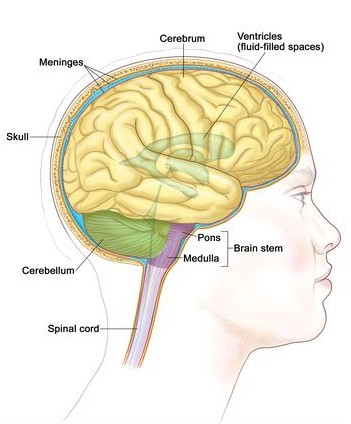
\includegraphics[width=0.55\textwidth]{brainanatomy.jpg}
    \caption{Depiction of some key regions of the brain reproduced from~\cite{Institute2023}.}
    \label{fig:anatomybrain}
\end{figure}
There are also different types of brain cells in which the tumour can originate. The brain contains many neurones which transport the electrical signals that allow the brain to operate. These are surrounded by glial cells, of which there are different types which each play a role in supporting and protecting the neurones~\cite{TheBrainTumourCharity2023}. The main types are astrocytes, oligodendrocytes and ependymal cells. When the tumour originates in glial cells it is termed a glioma with subcategories corresponding to each type of glial cell. Astrocytomas, originating in astrocytes, are the most common gliomas with the different grades given different names such as Grade 4 astrocytoma named glioblastoma multiforme~\cite{BrainTumourResearch2023}. Similarly, oligodendrogliomas originate from oligodendrocytes, and ependymomas originate from ependymal cells~\cite{TheBrainTumourCharity2023}. %include meningioma lymphoma medulloblastoma adenoma \\

There are over 130 types of brain tumours as classified by the World Health Organisation (WHO) and differ in terms of which type of cell they originate in, their grade, and which part of the brain they affect.

\subsection{Current treatments}\label{sec:introtumourtreatments}
Initially or if no other treatment options are possible, the symptoms of a brain tumour can be treated without treating the tumour itself, for example anti-sickness medication to treat the nausea. The treatment plans are determined based on a number of factors which include the type, location, and grade of the tumour as well as the patient's overall health~\cite{NationalHealthService2023}. Surgery is a preferred treatment where possible as it is possible to remove a large proportion, if not all, of the tumour with this method. In cases where the full tumour may not be removed, such as when there is a significant infiltration zone into surrounding healthy tissue where the border of the tumour is challenging to identify, this may be followed up with radiotherapy or chemotherapy. These treatment options can also be used separately when surgery is not an option~\cite{MacmillanCancerSupport2019}. 

Neurosurgical resection aims for maximum safe resection of the tumour which balances a high extent of resection while preserving functional regions of brain as improved resection is linked to improved patient outcomes~\cite{Chanbour2022}. To this end a variety of techniques can be employed to improve resection. These include: a surgical microscope which enables clear visualisation of the surgical field, neuronavigation which allows registration of a probe against an MRI, awake or asleep sub-corticol mapping to allow identification of eloquent areas of brain, in some cases fluorescence imaging or indocyanine green (ICG) can be used for tumour localisation, and microvascular doppler (MVD) or ICG can be used for tumour vessel localisation~\cite{Chanbour2022, Catapano2018}.
Whilst these these adjuncts have improved the quality of tumour resection, they are associated with some limitations~\cite{Chanbour2022}. Neuronavigation reduces in accuracy as the anatomy changes throughout a procedure. Whilst this can be counteracted using intra-operative MRI, this disrupts surgical workflow and has large associated costs~\cite{Chanbour2022}. Sub-cortical mapping allows identification of eloquent regions of brain, however this does not provide a spatially-resolved tumour boundary and carries risks of intraoperative seizures or postoperative emotional distress~\cite{Chanbour2022}. Label-based methods such as fluorescence and ICG can be effective but are limited by the label behaviour and the type of tumour in which it is effective~\cite{Chanbour2022}. Vessel localisation may also be effective with MVD or ICG displaying the flow of blood, however this is unable to quantify the oxygen saturation of this blood or verify the oxygen transfer into tissues which introduces an element of subjectivity into tissue viability assessment. 

This demonstrates the need to improve real-time, spatially-resolved, visualisation of tumour boundaries and vascularisation particularly for low-grade tumours where fluorescence imaging has limited application due to the low accumulation of fluorophore in these less aggressive tumours~\cite{Belykh2023, Kiesel2021}. 

\section{Brain aneurysms}
Brain aneurysms are a subset of all aneurysms which are balloon-like abnormal dilatation in a vessel wall due to a weakened caused by high blood pressure, smoking, or genetic predisposition~\cite{NationalHealthService2022}. Most aneurysms will only have significant sympoms on rupturing which is called a subarachnoid haemmorhage and can cause extensive brain damage as well as blinding headaches, sickness, or pain looking at light~\cite{NationalHealthService2022} with approximately 500,000 people dying annually~\cite{Toth2018}. 

\subsection{Current treatments}\label{sec:introaneurysmtreatments}
Treatment of unruptured aneurysm is determined by risk of rupture, size, and location in the brain. If the aneurysm is considered to have a low risk of rupture, treatment may focus on limiting risk factors~\cite{NationalHealthService2022}. In ruptured aneurysms or thos at higher risk of rupturing, however, treatment is primarily surgical in the form of clipping or endovascular procedures depicted in Figure \ref{fig:aneurysmtreatment}. The former involves the placement of a metal clip over the opening to prevent further blood flow into the aneurysm~\cite{TheBrainFoundation2023}. Endovascular procedures can include coiling to encourage clotting in the aneurysm to prevent further blood flow, which can be combined with further devices including stents to hold the coil in place~\cite{TheBrainFoundation2023}. The final endovascular technique is flow diversion achieved by placing a cylindrical tube (similar to a stent with a tighter weave) in the vessel over the aneurysm opening to allow normal blood flow~\cite{TheBrainFoundation2023}. 
\begin{figure}[h]
    \centering
    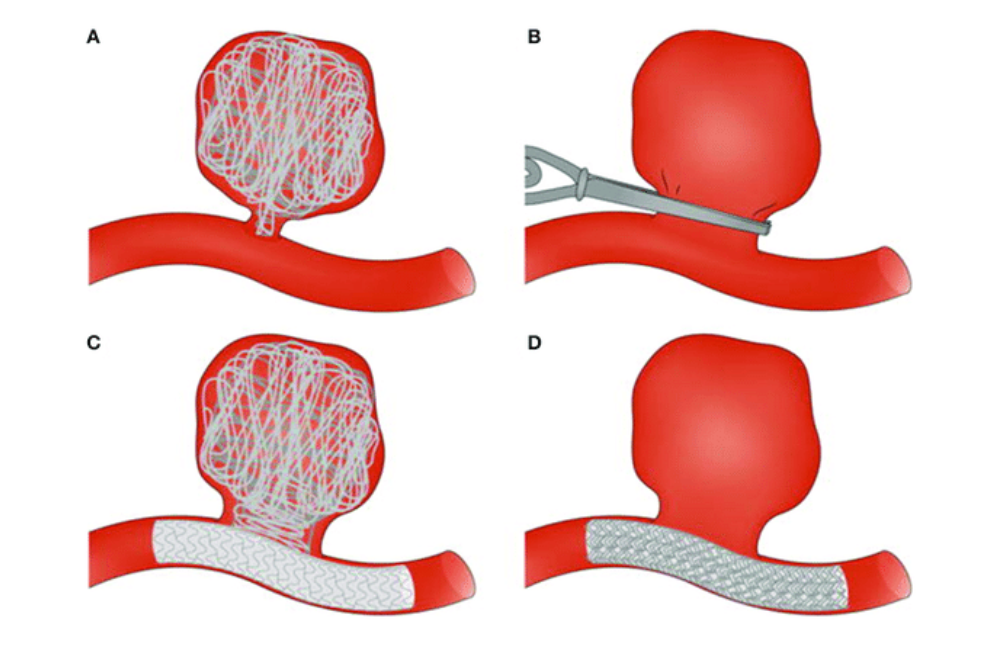
\includegraphics[width=0.9\textwidth]{Aneurysm-treatments.png}
    \caption{An illustration of some key surgical treatment methods for brain aneurysms reproduced from~\cite{TheBrainFoundation2023} where the technique depicted by A is coiling, B is clipping, C is coiling combined with a stent, and D is flow diversion.}
    \label{fig:aneurysmtreatment}
\end{figure}
Whilst these treatment methods are often very effective, incomplete aneurysm occlusion can lead to rupture at a later date with the extent of occlusion being linked to the likelihood of this occurring~\cite{Toth2018}. For this reason blood flow is often assessed intra-operatively using digital subtraction angiography (DSA), MVD, or ICG~\cite{Norat2019}. DSA is produced by subtracting an X-ray image taken without a contrast agent from one taken with a fluorescent contrast agent to visualise only the vessels in the field of view~\cite{Radiopia2022}. This can be done intra-operatively to visualise the blood flow, however the gold-standard for determining quality of aneurysm occlusion is a post-operative DSA~\cite{Marbacher2020}. DSA cannot be used continuously intra-operatively due to the changing geometry, the complex procedure for DSA aquisition, and the radiation dose risk~\cite{Radiopia2022, Derdeyn1999}. ICG provides a real-time alternative to DSA, however it also requires a fluorescent dye and is of lower precision~\cite{Norat2019, Anania2023}. MVD is also able to determine if full occlusion has occurred intra-operatively and has the advantage of not requiring a labelling agent, however this technique is highly subject to angle and depth~\cite{Anania2023}. This demonstrates that a real-time, label-free, spatially-resolved, quantitative demonstration of blood flow is currently unavailable. 
Additionally, temporary clipping of healthy vessels can be used to control intra-operative bleeding, however this may lead to cerebral ischaemia where tissues have limited access to oxygenated blood~\cite{Doron2022}. For this there is currently no intra-operative method of visualising oxygen saturation in these areas so a real-time, intra-operative, spatially-resolved, quantitative measure of oxygen saturation is desired. 

\section{Oxygen saturation}
Oxygen is required by all cells in the body to release energy by respiration. This oxygen is transported to cells by haemoglobin, primarily in the red blood cells of blood, which can take the forms of oxyhaemoglobin and deoxyhaemoglobin based on whether the haemoglobin is bound to oxygen or not respectively. These forms of haemoglobin have very different absorbance characteristics as seen in their extinction spectra in Figure \ref{fig:Haemoglobinext}. 
\begin{figure}[h]
    \centering 
    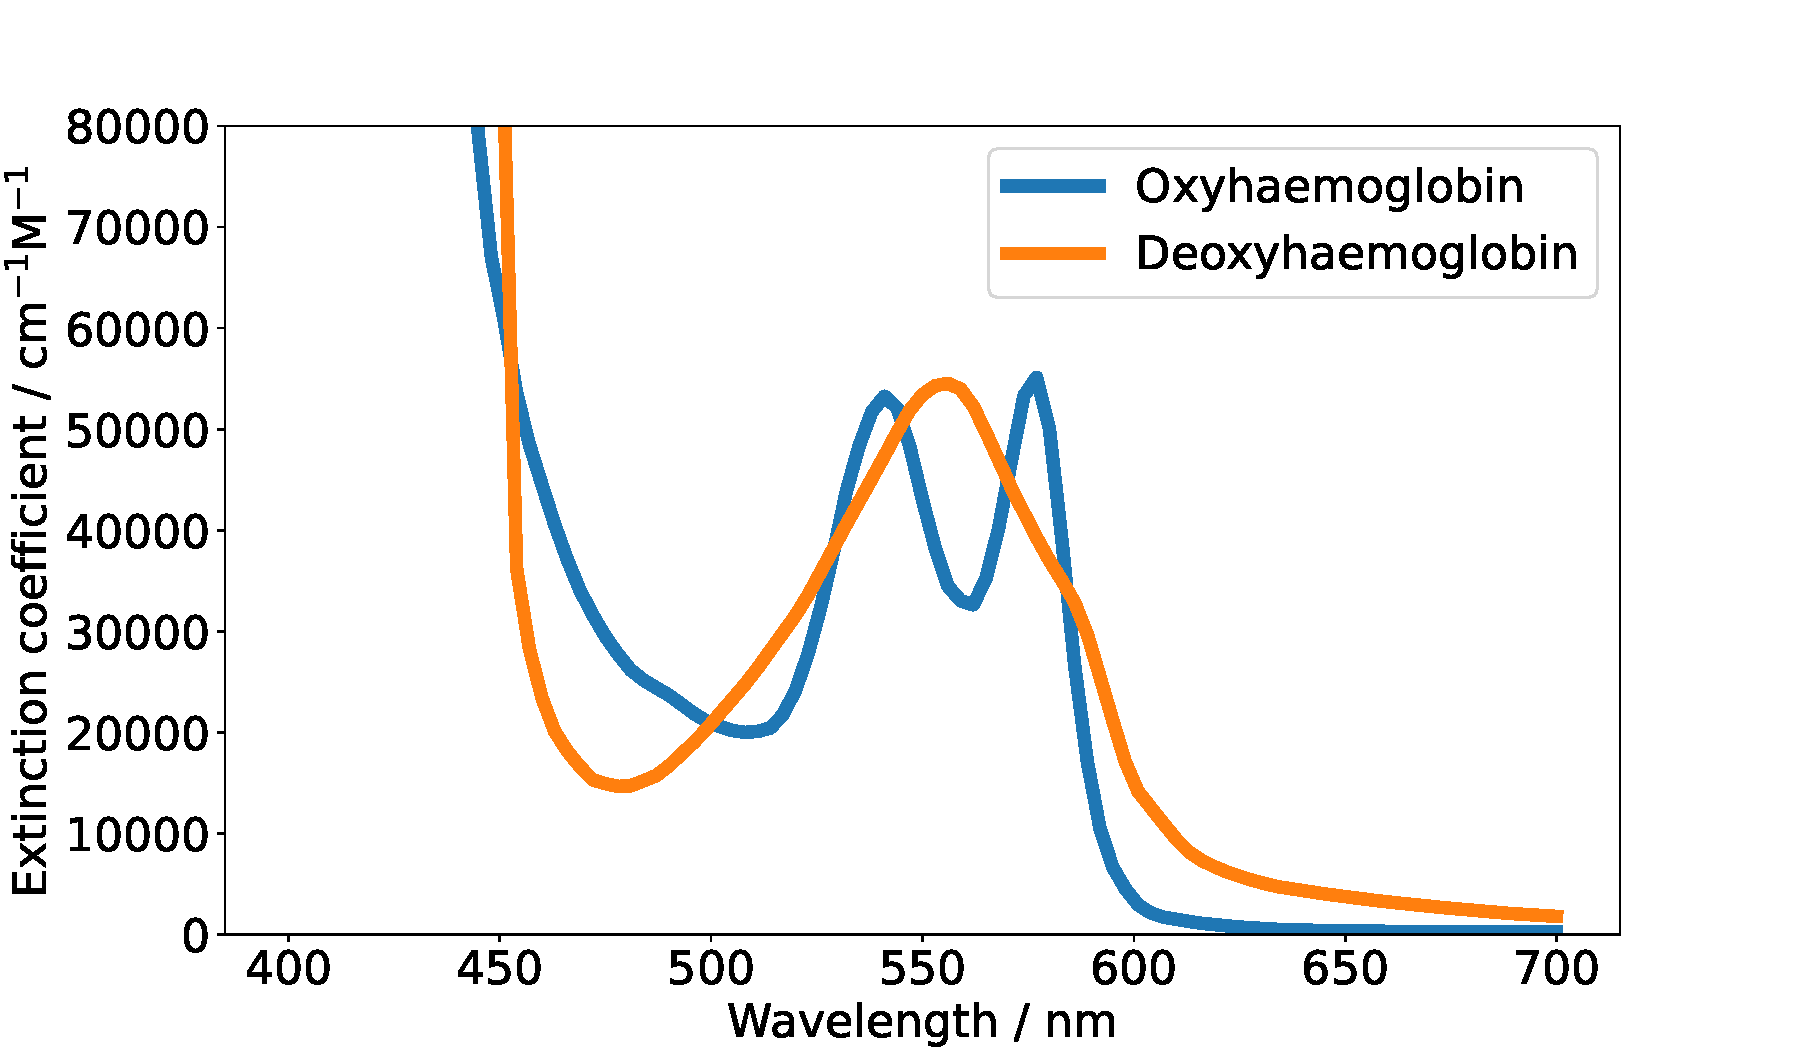
\includegraphics[width=0.7\textwidth]{Hb_eps.pdf}
    \caption{The extinction coefficients for oxyhaemoglobin and deoxyhaemoglobin reproduced from~\cite{Prahl1998}.}
    \label{fig:Haemoglobinext}
\end{figure}
Oxygen saturation is defined as the proportion of haemoglobin which is oxygenated ie $\frac{HbO_2}{HbO_2 + Hb}$ where $Hb$ is deoxyhaemoglobin and $HbO_2$ is oxyhaemoglobin. 

There are no currently established, intra-operative, techniques to assess $StO_2$ with respect to neurosurgery and so perfusion is often used as an indicator instead with DSA, MVD, and ICG capable of this as detailed in Sections \ref{sec:introtumourtreatments} and \ref{sec:introaneurysmtreatments}. Additionally, there has been significant research into using Laser Speckle Contrast Imaging (LSCI) to visualise blood perfusion, however this is not able to distinguish between $Hb$ and $HbO_2$ as yet~\cite{Dunn2012, Zhong2021}. Peri-operative neural monitoring can use jugular venous oxygen saturation (JVOS)~\cite{Raith2020} and cerebral oximetry~\cite{Lian2020} to provide indications of the health of the organ. Both techniques usually make use of near infra-red (NIR) spectroscopy to distinguish between $Hb$ and $HbO_2$. These techniques, however, lack specificity so local regions of ischaemia can be present when these values are within the bounds of normality~\cite{Raith2020, Zhong2021}.

Due to this lack of available techniques, there have been many proposed methods to extract $StO_2$ from tissue diffuse reflectance spectra. These range from the simplest ratiometric two-wavelength methods to more sophisticated analytical models~\cite{MacKenzie2018} or deep-learning based approaches~\cite{Ayala2023}. Using two or three wavelength models can provide good results but require data to be captured at these precise wavelengths placing large constraints on the measurement devices used and significant model assumptions, whereas analytical models can be applied to ranges of wavelengths for which they are developed. Alternatively, Monte Carlo methods are an established approach to modelling light-tissue interaction for a range of wavelengths. It is, however, computationally challenging to apply in an inverse problem setting making the estimation of optical properties from tissue spectra non trivial on the basis of Monte Carlo simulations alone. To obtain the diffuse reflectance spectra intra-operatively, these techniques primarily use HSI which enable non-contact imaging with minimal change to surgical workflow. 

\section{Outline of thesis}
In the current chapter I have outlined the principles of HSI and outlined the clinical need for an intra-operative, spatially-resolved, $StO_2$ method alongside the existing technology available for this. 
Chapter \ref{chap:SWB} investigates the necessity for in situ white references and address this by proposing a novel, sterile, synthetic reference construction algorithm. The use of references obtained at different distances and lighting conditions to the subject were examined. Spectral and color reconstructions were compared with standard measurements qualitatively and quantitatively, using $\Delta E$ and normalised RMSE respectively. The algorithm forms a composite image from a video of a standard sterile ruler, whose imperfect reflectivity is compensated for. The reference is modelled as the product of independent spatial and spectral components, and a scalar factor accounting for gain, exposure, and light intensity. Evaluation of synthetic references against ideal but non-sterile references is performed using the same metrics alongside pixel-by-pixel errors. Finally, intraoperative integration is assessed though cadaveric experiments.

Chapter \ref{chap:1layer} compares three analytical optical reflectance models for homogeneous, semi-infinite, tissue that have been proposed (Modified Beer-Lambert~\cite{Clancy2015}, Jacques 1999~\cite{Jacques1999}, Yudovsky 2009~\cite{Yudovsky2009}) which have not previously been directly compared for tissue parameter extraction purposes. I compare these analytical models using Monte Carlo simulated diffuse reflectance spectra and controlled gelatin-based phantoms with measured diffuse reflectance spectra and known ground truth composition parameters. 

In Chapter \ref{chap:2layer} a two layer model (Yudovsky 2009) is evaluated against Monte Carlo simulations and used to analyse a NIST skin reflectance dataset. By focussing on the quality of the oxygen saturation ($StO_2$) recovery, the performance of this model is evaluated across the parameter range and a significant region of failure identified. 

Chapter \ref{chap:HSImodel} investigates the impact of reducing the spectral resolution of the diffuse reflectance data and the introduction of noise by simulating camera responses from simulated and experimental data. This camera simulation is also used to adapt the analytical models for use with snapshot hyperspectral data. The impact of this is evaluated using simulations and gelatin-based phantom data similarly to previous chapters. This is evaluated using mean spectra from annotated regions of HSI images and on a pixel-by-pixel basis to investigate the ability of HSI to provide spatial resolution. Finally, some initial examples of applying these models to intra-operative, hyperspectral, neurosurgical data are shown. 